\documentclass[xcolor=dvipsnames]{beamer}
\usepackage[utf8]{inputenc} 
\usepackage[greek , english]{babel}
\usepackage{alphabeta}
\usepackage{graphicx}
\usepackage{hyperref}
\usetheme{Madrid}
\useoutertheme{miniframes} % Alternatively: miniframes, infolines, split
\useinnertheme{circles}

\definecolor{IITHorange}{RGB}{243, 130, 33} % UBC Blue (primary)
\definecolor{IITHyellow}{RGB}{254, 203, 10} % UBC Grey (secondary)

\setbeamercolor{palette primary}{bg=IITHorange,fg=white}
\setbeamercolor{palette secondary}{bg=IITHorange,fg=white}
\setbeamercolor{palette tertiary}{bg=IITHorange,fg=white}
\setbeamercolor{palette quaternary}{bg=IITHorange,fg=white}
\setbeamercolor{structure}{fg=IITHorange} % itemize, enumerate, etc
\setbeamercolor{section in toc}{fg=IITHorange} % TOC sections

% Override palette coloring with secondary
\setbeamercolor{subsection in head/foot}{bg=IITHyellow,fg=white}

\title[Προηγμένες Τεχνικές]{Παρουσίαση Προτζεκτ Προηγμένων Τεχνικών Προγραμματισμού\\
Forum}
\date{\today}
\institute[ΗΜΤΥ]{Κωνσταντόπουλος Κωνσταντίνος ΑΜ: 1066546\\
Λάμπρου Ευάγγελος ΑΜ: 1066519\\
Παπαδημητρίου Αποστόλης: 1066531\\
}

\begin{document}
    
    \begin{frame}
        \titlepage
    \end{frame}
    
    \begin{frame}
        \begin{center}
        \textbf{Code Quality}
        \end{center}
        \begin{itemize}
            \item Κοινός Formatter για τα μέλη της ομάδας
            \item Κοινό variable naming style
            \item Code Scanning με GitHub
        \end{itemize}
    \end{frame}

    \begin{frame}
        \begin{center}
        \textbf{Testing}
        \end{center}
        \begin{itemize}
            \item Χρήση της βιβλιοθήκης Jest
            \item Test για το api, db.
        \end{itemize}
        \begin{figure}[H]
            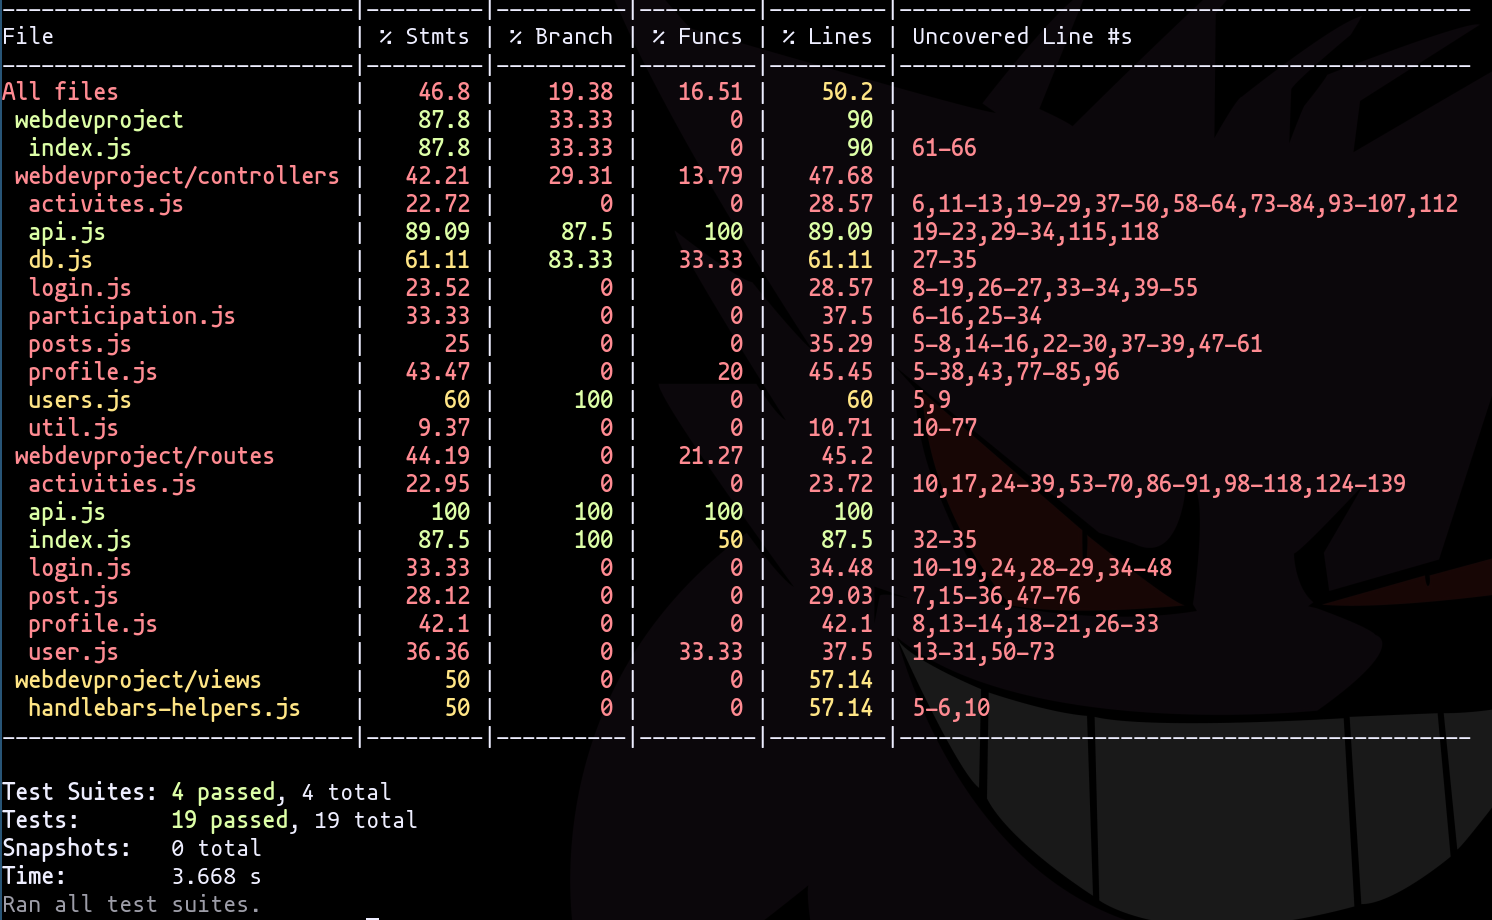
\includegraphics[width=0.4 \textwidth]{img/test1}
            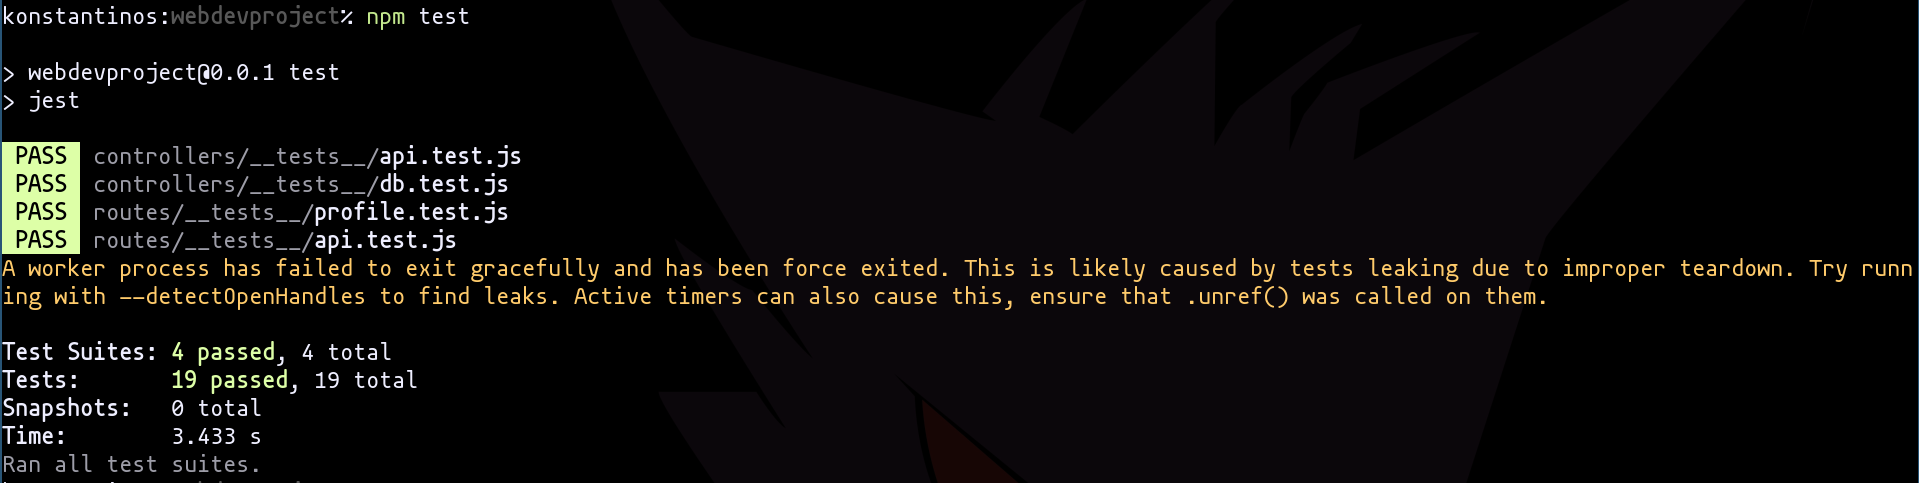
\includegraphics[width=0.4 \textwidth]{img/test2}
        \end{figure}
    \end{frame}
    \begin{frame}
        \begin{center}
        \textbf{Versioning}
        \end{center}
        \begin{itemize}
            \item GitHub
            \item \href{https://github.com/vagos/webdevproject}{Repo Link}
        \end{itemize}
        \begin{figure}[H]
            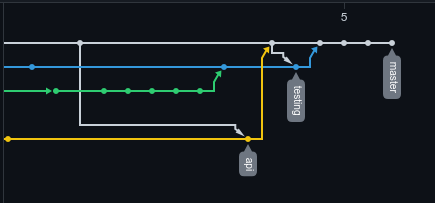
\includegraphics[width=0.4\textwidth]{img/branches}
            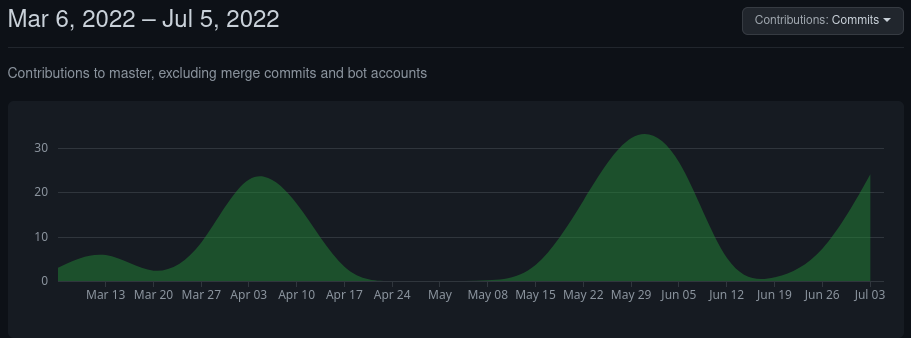
\includegraphics[width=0.4\textwidth]{img/insights2}
        \end{figure}
    \end{frame}
    % \begin{frame}
    %     \begin{figure}[H]
    %         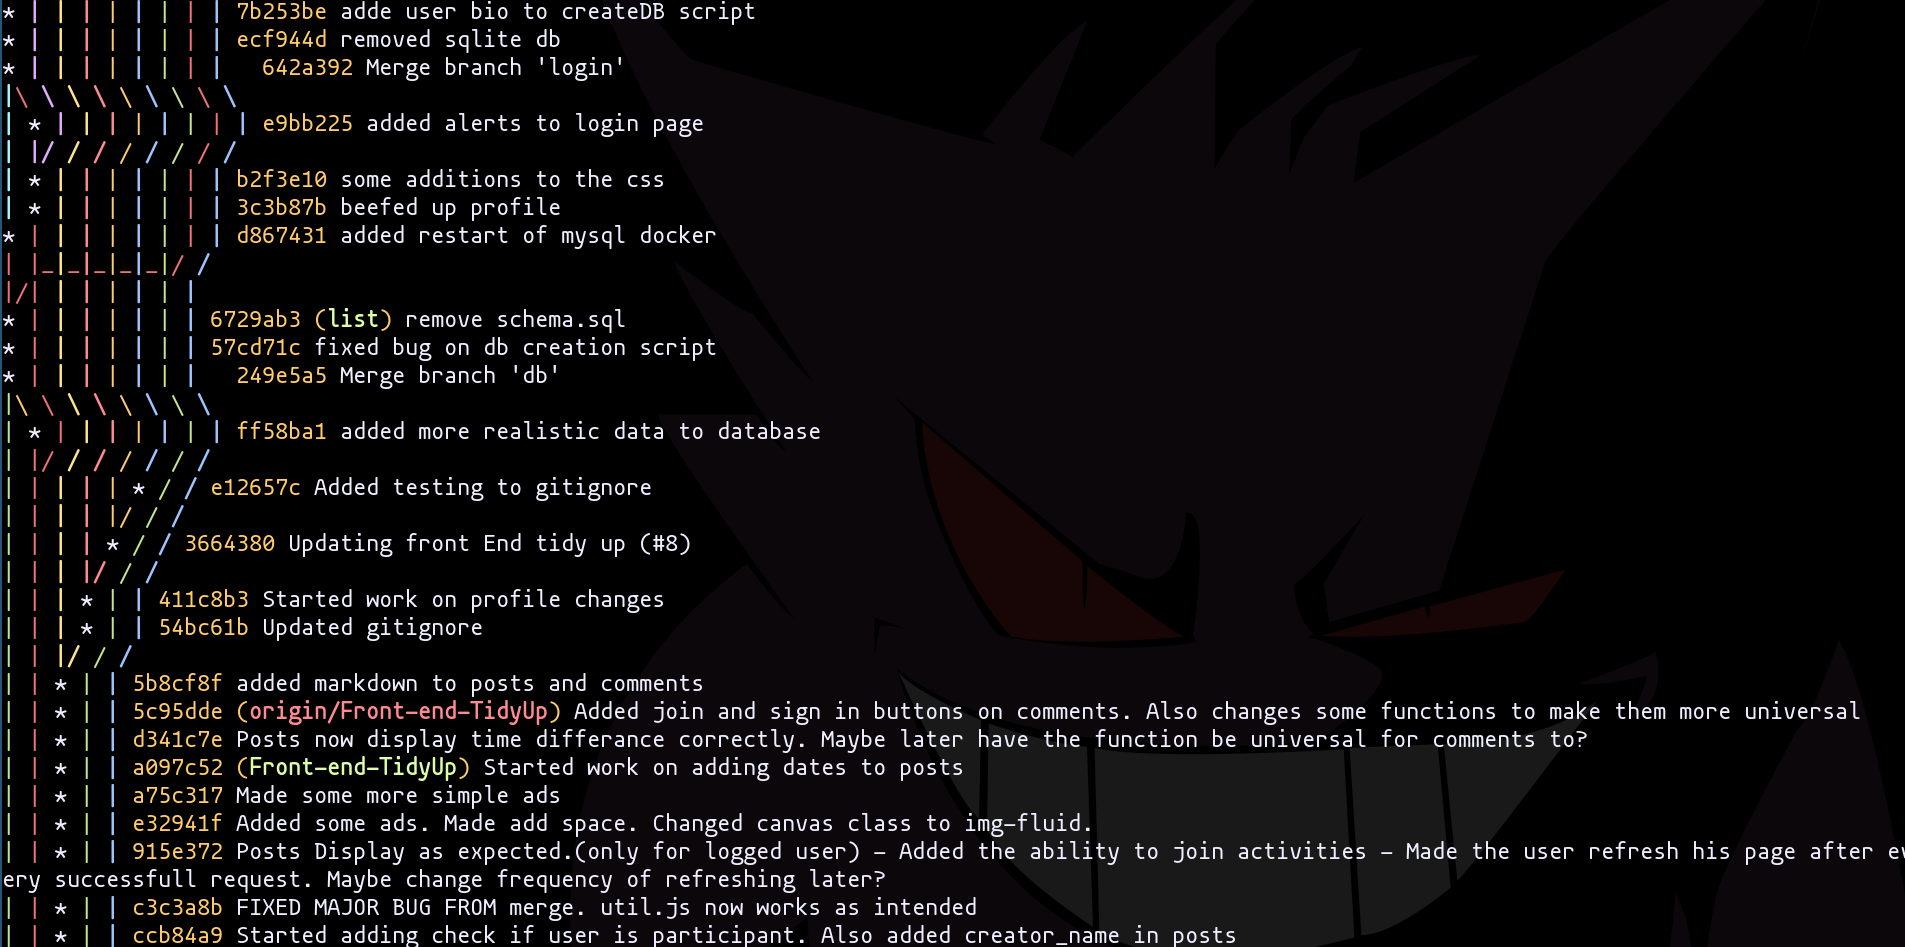
\includegraphics[width=0.4\textwidth]{img/graph1}
    %         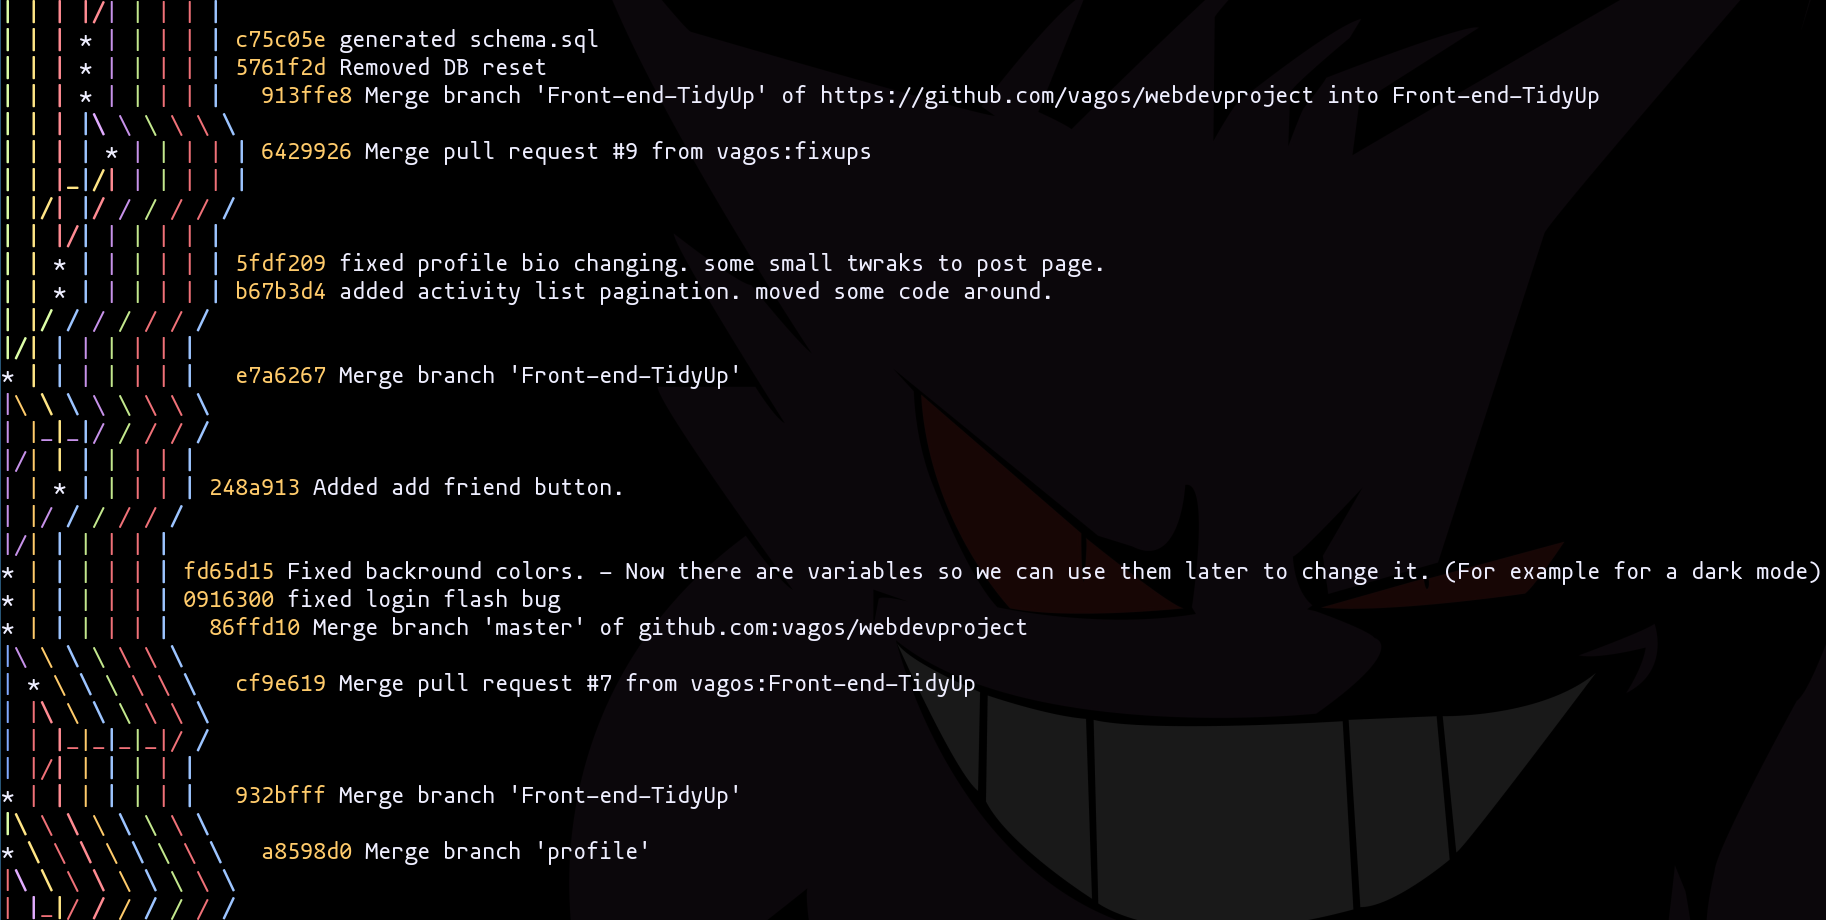
\includegraphics[width=0.4\textwidth]{img/graph4}
    %         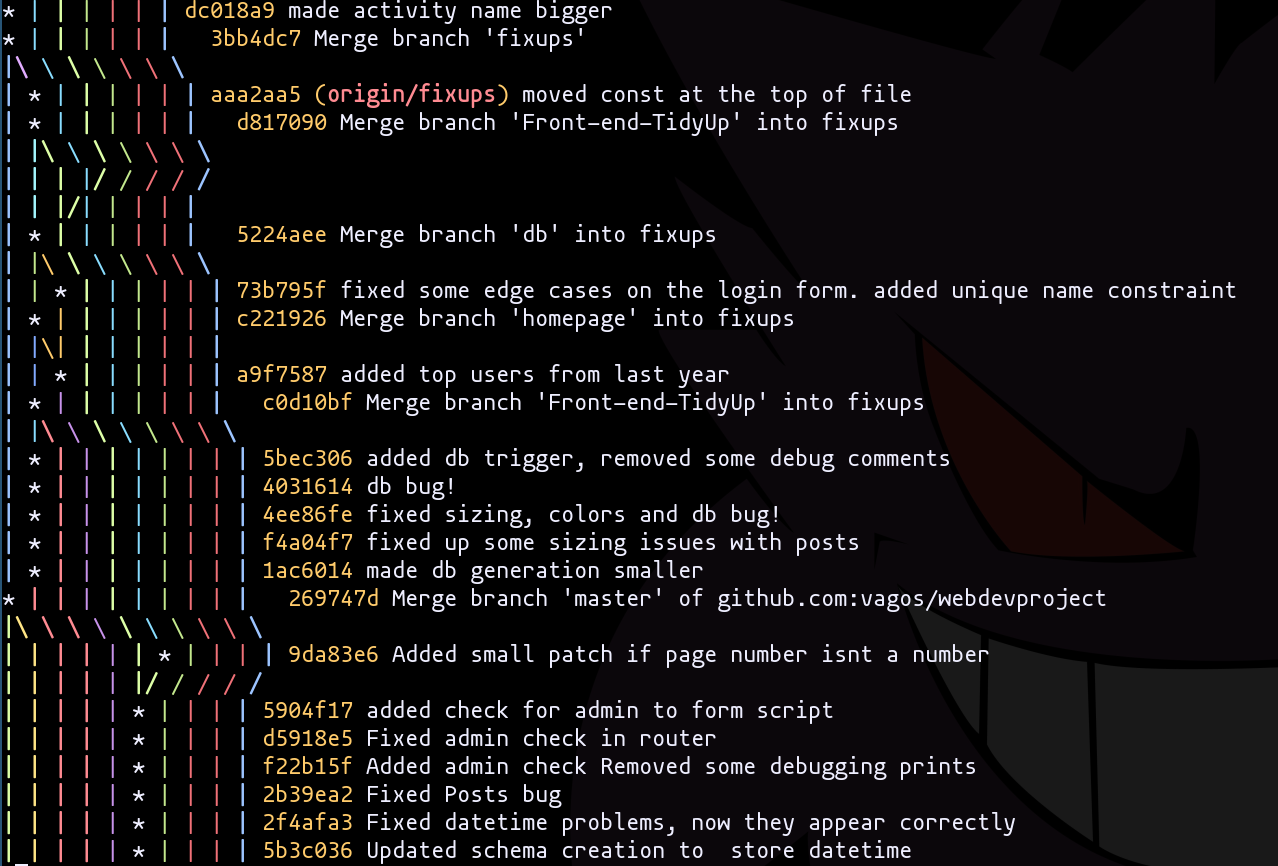
\includegraphics[width=0.4\textwidth]{img/graph3}
    %         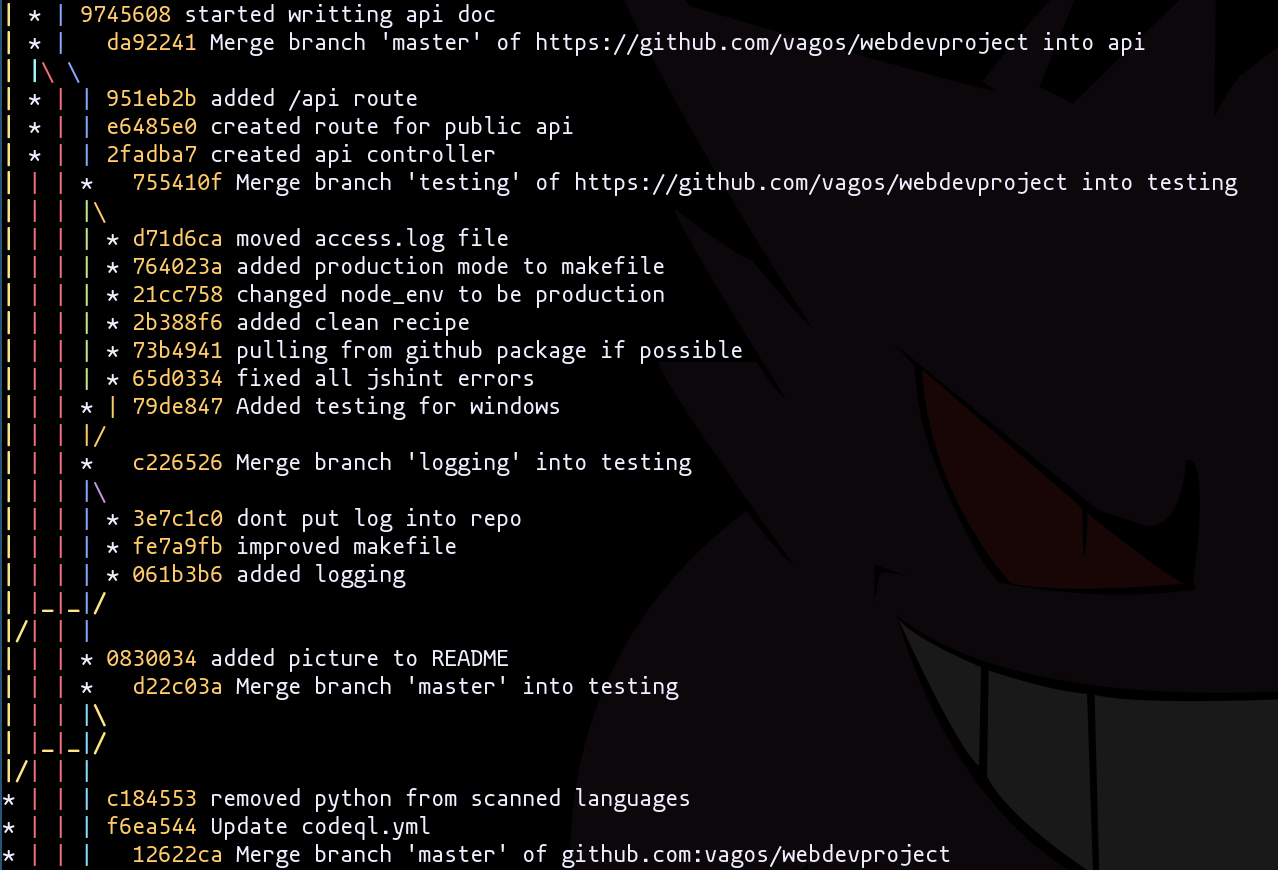
\includegraphics[width=0.4\textwidth]{img/graph2}
    %     \end{figure}
    % \end{frame}
    \begin{frame}
        \begin{center}
        \textbf{REST}
        \end{center}
        \begin{itemize}
            \item Δημιουργία API για GET requests
            \item Swagger για documentation του API
        \end{itemize}
    \end{frame}
    \begin{frame}
        \begin{center}
        \textbf{CI/CD}
        \end{center}
        \begin{itemize}
            \item GitHub Actions
            \item Έλεγχος με github workflows στα commits
            \item Έλεγχος με github actions στα push και merges
        \end{itemize}
    \end{frame}
    \begin{frame}
        \begin{center}
        \textbf{Virtualization}
        \end{center}
        \begin{itemize}
            \item Dockerize την εφαρμογή
        \end{itemize}
    \end{frame}
    \begin{frame}
        Ευάγγελος
        \begin{itemize}
            \item Docker
            \item Testing
            \item GitHub Actions CI/CD
            \item Code Linting
            \item Makefiles (Automatic Build System)
        \end{itemize}
        Αποστόλης
        \begin{itemize}
            \item Versioning
            \item FrontEnd
            \item FrontEnd-BackEnd Integration
            \item Testing 
            \item Makefiles
        \end{itemize}
        Κωνσταντίνος
        \begin{itemize}
            \item Docker
            \item Public API
            \item API Docs with Swagger
            \item Testing
        \end{itemize} 
    \end{frame}
\end{document}